\documentclass{llncs}
%
%\usepackage{makeidx}  % allows for indexgeneration
%\usepackage{amsthm,amsmath,amsfonts,amssymb}
\usepackage[locale=US]{siunitx}
\sisetup{binary-units=true}
\usepackage{graphicx}
\usepackage{subfig}
\graphicspath{{./figures/}}
\usepackage{booktabs}
%\usepackage{wrapfig}
\usepackage[table]{xcolor}
\usepackage{tikz}
\usetikzlibrary{arrows}
\usetikzlibrary{matrix}
%% \usetikzlibrary{shapes}
%% \usetikzlibrary{decorations.pathreplacing}
\usetikzlibrary{trees}
\usetikzlibrary{positioning}
\usepackage{algorithm}
\usepackage{algpseudocode}

% %%%%%%%%%%%%%%%%%%%%%%%%%%%%%%%%%%%%%%%%%%%%%%%%%%%%%%%%%%%%%%%%%%%%%%%%%%%%%%%
\usepackage{listings}
\lstset{numberbychapter=false} % listings absolute counter
\usepackage{textcomp}
% preserve ttdefault
\edef\oldtt{\ttdefault}
\usepackage[scaled]{beramono}
\usepackage[T1]{fontenc}
\renewcommand*\ttdefault{\oldtt}


\lstset{literate={~} {$\sim\,$}{1}}
\lstset{upquote=true}
\lstset{language=C++,
  basicstyle=\small\fontfamily{fvm}\selectfont,%\ttfamily,
% 	columns=fullflexible,
  columns=fixed,
  keepspaces=true,
%       keywordstyle=\color{black}\bf,
%       stringstyle=\color{red}\ttfamily,
  showstringspaces=false,
  commentstyle=\color[rgb]{0.3,0.3,0.3}\textit,
%       morecomment=[l][\color{gray}]{\#},
  identifierstyle=\color{black},
  morekeywords={size_t},
  emph={__global__,__device__},
        emphstyle=\textit,
        numbers=left,
  numberstyle=\small\color{gray},
  breaklines=true,
  numbersep=5pt,
  xleftmargin=.19in,
}
% %%%%%%%%%%%%%%%%%%%%%%%%%%%%%%%%%%%%%%%%%%%%%%%%%%%%%%%%%%%%%%%%%%%%%%%%%%%%%%%

\renewcommand*{\algorithmicrequire}{\textbf{Input:}}
\renewcommand*{\algorithmicensure}{\textbf{Output:}}

\newcommand{\todo}[1]{\textcolor{red}{(TODO #1)}}
\newcommand{\gearshifft}{\texttt{gearshifft}}
\newcommand{\mc}[1]{\lstinline!#1!}

\newcommand{\Title}{gearshifft -- The FFT Benchmark Suite for Heterogeneous Platforms}
%%%%%%%%%%%%%%%%%%%%%%%%%%%%%%%%%%%%%%%%%%%%%%%%%%%%%%%%%%%%%%%%%%%%%%%%%%%%%%%

\title{\Title}
%\subtitle{}
\titlerunning{gearshifft}
\toctitle{\Title}
\author{Peter Steinbach\inst{1} \and Matthias Werner\inst{2}}
\institute{Max Planck Institute of Molecular Cell Biology and Genetics,\\ 01307 Dresden, Germany,\\
\email{steinbac@mpi-cbg.de}
\and
Center for Information Services and High Performance Computing,\\
TU Dresden, 01062 Dresden, Germany\\
\email{Matthias.Werner1@tu-dresden.de}}

%%%%%%%%%%%%%%%%%%%%%%%%%%%%%%%%%%%%%%%%%%%%%%%%%%%%%%%%%%%%%%%%%%%%%%%%%%%%%%%

\usepackage[hyperfootnotes=false,bookmarks=false]{hyperref}
\hypersetup{
  pdftitle = {\Title},
  pdfsubject = {},
  pdfborder={0 0 0},
  colorlinks=false,
  linkcolor=[rgb]{0 0 0.3},
  urlcolor=[rgb]{0 0 0.3},
  citecolor=[rgb]{0 0 0.3},
  pdfauthor={Peter Steinbach, Matthias Werner},
  %plainpages=true
}
\usepackage[capitalize]{cleveref} % after hyperref

\usepackage[backend=biber,
citestyle=numeric-comp,
url=true,
natbib=true,
maxnames=3,
bibencoding=utf8,
sorting=nyt
]{biblatex}

% \bibliography{bibs}
% \bibliography{gearshifft_references}
\addbibresource{gearshifft_references.bib}

%%%%%%%%%%%%%%%%%%%%%%%%%%%%%%%%%%%%%%%%%%%%%%%%%%%%%%%%%%%%%%%%%%%%%%%%%%%%%%%
\pdfsuppresswarningpagegroup=1
%
\begin{document}
%
\frontmatter          % for the preliminaries
%
\pagestyle{headings}  % switches on printing of running heads
%\addtocmark{Hamiltonian Mechanics} % additional mark in the TOC

\maketitle              % typeset the title of the contribution

\begin{abstract}
  Fast Fourier Transforms (FFTs) are exploited in a wide variety of fields ranging from computer science to natural sciences and engineering. Most applications use frequency field information for filtering in a myriad of fashions. With the rising data production bandwidths of experimental hardware and modern simulations, judging best what algorithmic tool to apply, can be vital to any scientific endeavor. FFTs are no exception to this. Moreover, as tailored FFT implementations exist for an ever increasing variety of high performance computer hardware, choosing the best performing FFT implementation has strong implications for the hardware to purchase in the future, for resources FFTs consume and for possibly decisive financial and time savings ahead of the competition. We therefor present an open-source and vendor agnostic benchmark suite, called \gearshifft{}, to process a wide variety of problem sizes and types with state-of-the-art FFT implementations (FFTW, clFFT and cuFFT). \gearshifft{} allows for a reproducible, unbiased and fair comparison on a wide variety of hardware to explore which FFT variant is best for a given problem size.
\keywords{signal processing, FFT, fftw. cufft, clfft, GPU, GPGPU, benchmark, HPC}
\end{abstract}


\section{Introduction}
\label{sec:intro}
% - why gearshifft

Fast Fourier Transforms (FFTs) are at the heart of many signal processing and phase space exploration algorithms. Examples for their substantial usage come from image restoration in life sciences \cite{preibisch2014efficient,schmid2015real}, phase space reduction in weather forecasts \cite{maronga2015parallelized} to machine learning \cite{collobert2011torch7,jia2014caffe,abadi2016tensorflow} to just name a few.

As input data grows in size and variety both of experimental hardware \cite{huisken2004optical} and simulation outputs \cite{maronga2015parallelized}, input data on the order of Gigabytes to FFT libraries becomes the standard. With the advent of graphics processing units (GPUs) for scientific processing computing around the beginning of the 21st century and the subsequent availability of general purpose programming paradigms to program these \cite{du2012cuda}, vendor-specific and open-source libraries to perform FFTs on accelerators emerged (cuFFT \cite{nvidia2010cufft} by nVidia, open-source clFFT \cite{clfft}) to offer performance which supersedes traditional high-performance implementations running on standard Central Processing Units (CPUs) such as the open-source fftw library \cite{FFTW97,FFTW05} or the intel specific MKL \cite{intel2007intel}.

However, a top ten sites listed among the fastest worldwide (top500 \cite{meuer2011top500}) shows that the used hardware is by far not homogenous. 


% - what has been done
% - status of gearshifft dev



\section{Motivation}
\label{sec:motivation}
A FFT is a fast implementation of the discrete Fourier transform which is a standard text-book mathematical procedure. The forward transform is a mapping from an array $x$ of $n$ complex numbers in the time domain to an array $X$ of $n$ complex numbers in the frequency domain (also referred to as Fourier domain):
%
\begin{equation}
  \label{eq:dft}
  X[k] = \sum_{j=0}^{n-1} x[j]e^{\frac{-2\pi\sqrt{-1}jk}{n}}
\end{equation}
%
with $k$ being an integer index within $0 \le k < n$. This operation was found to be computable in $\mathcal{O}(n \log n)$ complexity by Cooley-Turkey \cite{cooley1965algorithm}, which in turn rediscovered findings by Gauss \cite{gauss}. The basis the Cooley-Turkey approach is the observation that, given the factorization of $n=n_1n_2$, the  DFT of size $n$ can be rewritten by smaller DFTs of size $n_1$ and $n_2$. Given the aforementioned indices $j=j_1n_2 + j_2$ and $k=k_1+k_2n_1$, \cref{eq:dft} can be re-expressed as:
%
\begin{equation}
  \label{eq:cooley-turkey}
  X[k_1{+}k_2n_1] = \sum_{j_2=0}^{n_2-1} \left( \left( \sum_{j_1=0}^{n_1-1} x[j_1n_2{+}j_2] e^{\frac{-2\pi\sqrt{-1}j_1k_1}{n_1}} \right) e^{\frac{-2\pi\sqrt{-1}j_2k_1}{n}} \right) e^{\frac{-2\pi\sqrt{-1}j_2k_2}{n_2}}
\end{equation}

\cref{eq:cooley-turkey} describes a decomposition that can be performed recursively \cite{FFTW05}. Here, $n_1$ is denoted \emph{radix} as it refers to $n_1$ transforms of size $n_2$. These smaller transforms are combined by a \emph{butterfly} graph with $n_2$ DFTs of size $n_1$ on the outputs of the corresponding sub-transforms. Radix-2 DFTs ($n$ being a power of two) are mostly implemented with the Cooley-Tukey algorithm \cite{cooley1965algorithm}. Stockham's formulations of the FFT can be applied \cite{stockham1966high} to avoid incoherent memory accesses. Arbitrary and mixed radices are more complicated and can be tackled with the prime-factorization or Chirp Z-transform implemented by the Bluestein's algorithm \cite{bluestein}. 

As \cref{eq:cooley-turkey} (similar to \cite{bluestein,stockham1966high}) can be considered a specialization of \cref{eq:dft}, the latter can be used to approximate the algorithmic complexity, i.e. a ratio of compute operations per accessed byte of memory. \cref{eq:dft} is a reduction of single- or double-precision floating point numbers \cite{ieee2008754}. A reduction of single-precision inputs on a fused multiply-add architecture (i.e. 1 addition and 1 multiplication in one instruction) would imply 1 operation per $\SI{4}{\byte}$ accessed and hence an arithmetic complexity of $1/4$ which would be a memory bound operation. As the exponentiation is not encoded into a single x86 instruction on any known architecture, it has to be expressed as a combination of \mc{FYL2X} and \mc{F2XM1}. On Intel Haswell, each of these instructions on scalar inputs consume at least $55\,\mu\text{ops}$ or $58\,\mu\text{ops}$ \cite{agnerfog} and it is hard if not impossible to estimate on paper how many cycles the entire exponentiation will consume. However, we can state that the exponentiation of floating point inputs will be compute bound. To summarize, this implies that \cref{eq:dft} and variations thereof will exhibit a compute bound performance profile where the cost of memory access is negligible (all required data is in the cache) and that this operation is memory bound elsewhere.  

Given the multitude of mathematical formulations and the heterogeneity of hardware, \gearshifft{} approaches the challenge of benchmarking a variety of FFT libraries from a user perspective. This means, that the following parameters shall be easy to study:

\begin{itemize}
\item FFT dimension and radix-type (e.g. $32{\times}32{\times}32$ as radix-2 3D FFT)
\item transform kinds, i.e. real-to-complex or complex-to-complex transforms
\item precision, i.e. 32-bit or 64-bit IEEE floating point number representation
\item memory mode
  \begin{itemize}
  \item \emph{in-place}: the input data structure is used for storing the output data (low memory footprint and low bandwidth are to be expected)
  \item \emph{out-of-place}:  where the transformed input is written to a different memory location than where the input resides (high memory footprint and high bandwidth are to be expected)
  \end{itemize}
\item transform direction, i.e. forward (from discrete space to frequency space) or backward (from frequency space to discrete space)
\end{itemize}
 


\section{Implementation}
\label{sec:implementation}

% - [open source] framework: c++14 with help of boost
% - demonstrate usage of gearshifft framework
% - cufft, clfft, fftw
% - issues?
% - #runs, cmake, project structure
% - libraries : mem checks

\gearshifft{} is developed as an open-source framework using C++14 standard and Boost Unit Test Framework for managing the benchmark trees.
The frontend API is basically just a wrapper mapping the use case explained in \cref{sec:benchmark_model}.
This interface is designed to integrate any given FFT library, that provides forward and backward Fourier transforms.
The wrapper code leverages C++ templates and compile-time constant expressions.
This yields minimal overhead at runtime and provides a type-agnostic interface, i.\,e. it is not fixed to single or double precision.
However, corresponding timer calls and benchmark routines for collecting data are required at runtime, so measurements will have to be verified.

The frontend interface requires the user to implement the context class and a class with implementation of FFT routines.
The context class in \cref{lst:implcontext} is instantiated only once for the application lifetime.
FFT implementation class in \cref{lst:implfft} is instantiated once per benchmark run and follows the ``resource allocation is initialization'' (RAII) pattern.


\begin{lstlisting}[caption={Context class required by gearshifft API},label={lst:implcontext}]
struct Context {
  /// title for all benchmarks
  static std::string title();
  /// list all compute devices
  static std::string getListDevices();
  /// information for current device
  std::string getDeviceInfos();
  /// creates context
  void create();
  /// destroys context
  void destroy();
};
\end{lstlisting}
\begin{lstlisting}[caption={FFT class required by gearshifft API},label={lst:implfft}]
template<
 typename TFFT, // e.g. gearshifft::FFT_Inplace_Real, ...
 typename TPrecision, // e.g. double, float, ...
 size_t   NDim        // 1,..,3
>
struct MyImpl {
  MyImpl();
  ~MyImpl();
  void malloc();
  size_t getAllocSize();
  size_t getTransferSize();
  size_t getPlanSize();
  void init_forward();
  void init_backward();
  void execute_forward();
  void execute_backward();
  template<typename THostData>
  void upload(THostData* input);
  template<typename THostData>
  void download(THostData* output);
  void destroy();
};
\end{lstlisting}
\begin{lstlisting}[caption={Using FFT class},label={lst:implfftusing}]
using Inplace_Real =
gearshifft::FFT<gearshifft::FFT_Inplace_Real, MyImpl, TimerCPU>;
\end{lstlisting}

The wrapper for the user FFT class and the layout of measurement is given in the \lstinline!gearshifft::FFT! class.
Its are shown in \cref{lst:fftabstract}. The measurement framework is illustrated in \cref{fig:timings}.
\begin{lstlisting}[caption={FFT wrapper class},label={lst:fftabstract}]
template<
 typename TFFT,
 template <typename,typename,size_t,typename... > typename TPlan,
 typename TDeviceTimer,
 typename... TPlanArgs // is redirected to TPlan
>
struct FFT : public TFFT {
  template<typename T_Result, typename T_Vector, size_t NDim>
  void operator(/*..*/);
};
\end{lstlisting}

% implies plan reuse
\begin{figure}\label{fig:timings}
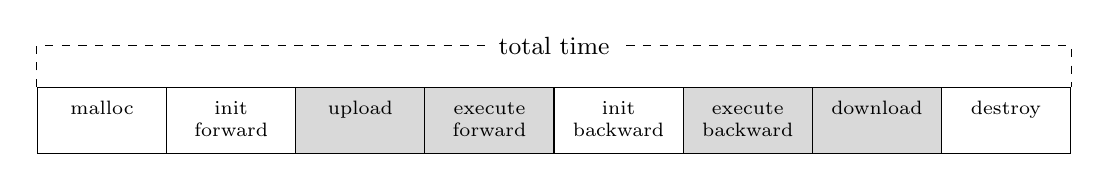
\begin{tikzpicture}
\tikzset{gr1/.style={fill=black!15}}
\matrix[
 minimum height=1.5em,
 matrix of nodes,
 row sep=-\pgflinewidth,
 column sep=-\pgflinewidth,
 text depth=2.5ex,
 text height=1.5ex,
 text width=4em,
 align=center,
 nodes in empty cells,
 row 1/.style={nodes={rectangle,draw,minimum width=3em,font=\scriptsize}}
]
(mf) at (0,0) {
malloc &
init\linebreak forward &
|[gr1]| upload &
|[gr1]| execute\linebreak forward &
init\linebreak backward &
|[gr1]| execute\linebreak backward &
|[gr1]| download &
destroy\\
};
\draw[dashed] (mf-1-1.north west) -- ++(0,1.5em) -| (mf-1-8.north east) node[pos=0.25,fill=white,font=\small] {total time};
\end{tikzpicture}
 \caption{Each operation is measured, where the colored ones are measured by device timers if required.}
\end{figure}


The backend of \gearshifft{} uses Boost Unit Test Framework to manage the benchmark instances.



\section{Results}
\label{sec:results}
Based on the experiences made for \cite{preibisch2014efficient, schmid2015real}, this section will discuss results obtained with \gearshifft{} on various hardware in order to showcase the capabilities of \gearshifft{}. We will assume the motivation of a developer seeking to optimize the use of FFTs in the context of the aforementioned publications, i.e. 3D real-to-complex transforms with contiguous single-precision input data. If not stated otherwise, this is the transform type assumed for all illustrations hereafter. 

Expeditions into other use cases will be made where appropriate. The curious reader may rest assured that a more comprehensive study is possible with \gearshifft{}, however the mere multiplicity of all possible combinations and use cases of FFT render it neither feasible nor practical to discuss all of them here.

For this study, we will concentrate on three modern and current FFT implementations available free of charge: \fftw{} ($3.3.5$, on x86 CPUs), \cufft{} ($8.0.44$, on nVidia GPUs) and \clfft{} ($2.12.2$, on x86 CPUs or nVidia GPUs). We consider this the natural starting point of developers beyond possible domain specific implementations. It should be noted, that this will infer not only a study in terms of hardware performance, but also how well the APIs designed by the authors of \fftw{}, \clfft{} and \cufft{} can be used in practice. 

\subsection{Experimental Environment}
\label{ssec:env}

The results presented in the following sections were collected on three systems:

\begin{table}[tbp]
  \centering
  \caption{Benchmark Hardware}
  \label{tab:hardware}
  \begin{tabular}{lllll}
    \toprule
                        & \multicolumn{2}{c}{\textbf{Taurus}}           & \textbf{Hypnos}           & \textbf{Islay}                                  \\
                        & \multicolumn{2}{c}{HPC Cluster \cite{taurus}} & HPC Cluster \cite{hypnos} & Workstation                                     \\
    \midrule
    \textbf{CPU family} & Haswell Xeon                                  & Sandybridge Xeon          & Haswell Xeon           & Haswell Xeon           \\
    \textbf{CPU model } & $2{\times}$ E5-2680 v3                        & $2{\times}$ E5-2450       & $2{\times}$ E5-2603 v3 & $2{\times}$ E5-2640 v3 \\
    \textbf{RAM       } & \SI{64}{\gibi\byte}                           & \SI{48}{\gibi\byte}       & \SI{64}{\gibi\byte}    & \SI{64}{\gibi\byte}    \\
    \textbf{GPU family} & Tesla                                         & Tesla                     & Tesla                  & GeForce                \\
    \textbf{GPU       } & 4x K80                                        & 2x K20x                   & 1x P100                & 1x GTX 1080            \\
    \textbf{GPU memory} & 4x \SI{12}{\gibi\byte}                        & \SI{6}{\gibi\byte}        & \SI{16}{\gibi\byte}    & \SI{8}{\gibi\byte}     \\
    \textbf{GPU driver} & $367.48$                                      & $367.48$                  & $367.48$               & $367.57$               \\
    \textbf{OS}         & RHEL $7.2$                                    & RHEL $7.2$                & Ubuntu $14.04.3$       & CentOS $7.2$           \\
    \bottomrule
  \end{tabular}
\end{table}

All systems presented in \cref{tab:hardware} will be used for the benchmarks in this section. Access was performed via a \texttt{ssh} session without running a graphical user interface running on the target system. All measurements used the GNU compiler collection (GCC) version 5.3.0 as the underlying compiler if not stated otherwise. All used GPU implementations on nVidia hardware interfaced with the proprietary driver listed in \cref{tab:hardware} and used the infrastructure provided by CUDA $8.0.44$ if not stated otherwise. 

Each benchmark is executed five times. From this, the arithmetic mean and sample standard deviations are used for figures presented below. As the number of repetitions is a configurable parameter of \gearshifft{}, we leave it to the user to produce a more comprehensive data set than used for this publication. We consider five repetitions enough at this point to show and discuss several aspects of performance and usability of \gearshifft{} and the FFT libraries under study.  

\subsection{Time To Solution}
\label{ssec:tts}

We begin the discussion with the classical use case for developers that might be accustomed to small size transforms. As such, an out-of-place transform with \texttt{powerof2} signal shapes will be assumed. The memory volume required for this operation amounts to the real input array plus an equally shaped complex output array of the same precision.   

\begin{figure}[!htbp]
  \centering
  \includegraphics[width=\textwidth]{figures/results_tts_legend.pdf}\vspace{-1em}
  \subfloat[linear scale]{\includegraphics[width=0.45\textwidth]{figures/results_tts_a.pdf}\label{fig:tts_a}}
  \hfill
  \subfloat[log10-log2 scale]{\includegraphics[width=0.45\textwidth]{figures/results_tts_b.pdf}\label{fig:tts_b}}
  \caption{Time-to-solution for power-of-2 3D single-precision real-to-complex forward transforms using \fftw{} (\mc{FFTW_ESTIMATE}) and \cufft{}. \cref{fig:tts_b} shows the same data as \cref{fig:tts_a} but in a log10-log2 scale.}
  \label{fig:tts}
\end{figure}

\cref{fig:tts} reports a comparison of runtime results of power-of-2 single-precision real-to-complex forward transforms from \fftw{} and \cufft{}. It is evident that given the largest device memory available of  \SI{16}{\gibi\byte}, the GPU data does not yield any points higher than \SI{8}{\gibi\byte}. Note that the total time reflects the time described in \cref{fig:framework}, i.e. it is the sum of the time to set up a plan, allocate memory on device, perform the data transfer onto the device, execute the FFT, transfer the result back to the host and clean up the used plan and the allocated memory. \cref{fig:tts_a} shows that the oldest GPU generation used in this comparison yields the slowest results for input signals in the order of \SIrange{1}{2}{\gibi\byte}. All other and more recent GPU models supersede \fftw{} using all available cores a $2\times12\,\text{core}$ double socket Intel Haswell CPU. Any judgment on the superiority of \cufft{} over \fftw{} can be considered premature at this point, as \fftw{} was used with the \mc{FFTW_ESTIMATE} planner flag.

\begin{figure}[!htbp]
  \centering
  \includegraphics[width=\textwidth]{figures/results_plan_flags_legend.pdf}\vspace{-1em}
  \subfloat[time to solution]{\includegraphics[width=0.45\textwidth]{figures/results_plan_flags_a.pdf}\label{fig:plan_flags_a}}
  \hfill
  \subfloat[time for forward transform only]{\includegraphics[width=0.45\textwidth]{figures/results_plan_flags_b.pdf}\label{fig:plan_flags_b}}
  \caption{Time-to-solution for power-of-2 3D single-precision real-to-complex inplace forward transforms using \fftw{} (\mc{FFTW_ESTIMATE}) and \cufft{}. \cref{fig:plan_flags_a} report the complete time to solution, whereas \cref{fig:plan_flags_b} is limited to the time spent for the execution of the forward transform only. Both figures use a log10-log2 scale.}
  \label{fig:fftw_plan_flags}
\end{figure}

\cref{fig:fftw_plan_flags} compares the time-to-solution to the actual time spent for the FFT operation itself. This illustration makes the cost and the benefit of higher planning flags than \mc{FFTW_ESTIMATE} obvious. \mc{FFTW_MEASURE} imposes a total runtime penalty of 1 to 2 orders of magnitude with respect to \mc{FFTW_ESTIMATE}, but it offers superior performance if limited to pure FFT execution timings compared \mc{FFTW_ESTIMATE}. For illustration, we generated the wisdom for shapes up to $64\times64\times64$ elements. As during plan creation, the \emph{wisdom} has to be loaded from disk only, the planning times are drastically reduced and \cref{fig:plan_flags_b} shows that the user is rewarded by pure FFT runtimes of less than an order of magnitude for small signal sizes. However, the FFT runtimes become even larger than those of \mc{FFTW_ESTIMATE} for input signal sizes of more than \SI{32}{\kibi\byte}. So a consequent use of \fftw{} \emph{wisdom} cannot be recommended to developers. 

It must emphasized that the planning times for \mc{FFTW_MEASURE} become prohibitively large for large input data sizes and reach minutes for data sets in the Gigabyte range. This is a well-known feature of \fftw{} as the authors note in \cite{FFTW05}:
%
\begin{quote}
  ``In performance critical applications, many transforms of the same
  size are typically required, and therefore a large one-time cost is
  usually acceptable.''
\end{quote}
% 
\gearshifft{} allows to dissect this problem further and isolate the planning time only.
%
\begin{figure}[!tbp]
  \centering
  \includegraphics[width=\textwidth]{figures/results_plan_time_legend.pdf}\vspace{-1em}
  \subfloat[3D transforms]{\includegraphics[width=0.45\textwidth]{figures/results_plan_time_a.pdf}\label{fig:plan_time_a}}
  \hfill
  \subfloat[1D transforms]{\includegraphics[width=0.45\textwidth]{figures/results_plan_time_b.pdf}\label{fig:plan_time_b}}
  \caption{Time-to-plan for power-of-2 single-precision inplace real-to-complex forward transforms using \fftw{}, \cufft{} and \clfft{}. \cref{fig:plan_time_a} reports the complete time to plan for 3D transforms, whereas \cref{fig:plan_time_b} is limited to 1D transforms. ``None'' refers to the planning with cufft as it does not support the plan rigor concept. Both figures use a log10-log2 scale.}
  \label{fig:plan_time}
\end{figure}
%
\cref{fig:plan_time} illustrates the problem to it's full extent. \mc{FFTW_MEASURE} consumes up to 3-4 orders of magnitude more time to produce a plan than a standard (GPU based libraries) or \mc{FFTW_ESTIMATE} based planner call especially for large input shapes, see \cref{fig:plan_time_a}. We compare the 3D planning with it's counterpart in 1D (see \cref{fig:plan_time_b}). It is important to note that \fftw{} planning in 1D appears to be very expensive in terms of plan time as the \mc{FFTW_MEASURE} curve is very steep compared to \cref{fig:plan_time_a}. At input sizes of \SI{128}{\mebi\byte} in 1D, the planning phase exceeds the duration of \SI{100}{\second}. In practice, this imposes a challenge on the client to the \fftw{} API. Not only is the time to solution affected by this behavior which is a crucial quantity if FFT-heavy applications are run. Moreover, in an HPC environment the runtime of applications needs to be known before executing them in order to allow efficient and rapid job placement on compute resources. From a nother perspective, this asserts a development pressure on the developer interfacing with \fftw{} as she has to create infrastructure (thread-safe static objects or similar come to mind) in order to perform the planning of \fftw{} only once and reuse the resulting plan as much as possible.

\subsection{Comparing CPU versus GPU runtimes}
\label{ssec:cpu_vs_gpu}

The last section finished by discussing a design artifact, that the \fftw{} authors introduced in their API and which other FFT libraries adopted. Another important question typically asked is if GPU accelerated FFT implementations are really faster than their CPU equivalents. Although this question cannot be answered comprehensively in our study, we would like to point out several aspects of it. First of all, modern GPU are connected via the PCIe bus to the host system in order to transfer data, receive instructions and to be supplied with power. This imposes a severe bottleneck to data transfer and is sometimes neglected during library design. Therefor, the time for data transfer needs to be accounted for or removed from the measurement. \gearshifft{}s results data model offers access to each individual step of a transformation, see \cref{fig:framework}. With it, it is possible to isolate the time for the FFT transform only.

\begin{figure}[!tbp]
  \centering
  \includegraphics[width=\textwidth]{figures/results_r2c_fwd_legend.pdf}\vspace{-1em}
  \subfloat[3D transforms]{\includegraphics[width=0.45\textwidth]{figures/results_r2c_fwd_a.pdf}\label{fig:r2c_fwd_a}}
  \hfill
  \subfloat[1D transforms]{\includegraphics[width=0.45\textwidth]{figures/results_r2c_fwd_b.pdf}\label{fig:r2c_fwd_b}}
  \caption{Time for computing power-of-2 single-precision real-to-complex forward transforms using the 3D API (\cref{fig:r2c_fwd_a}) and the 1D API \clfft{} (\cref{fig:r2c_fwd_b}). Both figures use a log10-versus-log2 scale.}
  \label{fig:r2c_fwd}
\end{figure}

\cref{fig:r2c_fwd} shows the runtime spent for computing the forward FFT for real single precision input data. This illustration is a direct measure for the quality of the implmentation and the hardware underneath. For the 3D case in \cref{fig:r2c_fwd_a}, we see that at the time of writing, \fftw{} on a double socket Haswell Intel Xeon E5 CPU provides very compelling performance if the input data is not larger than \SI{1}{\mebi\byte}. Above this limit, the GPU implementations offer a clear advantage by up to one order of magnitude. The current Pascal generation GPUs used with \cufft{} provide the best performance, which does not come by surprise as both cards are equipped with GDDR5X or HBM2 memory which are clearly beneficial for an operation that yields low computational complexity such as the FFT, see \cref{sec:motivation}. In the 1D case of \cref{fig:r2c_fwd_b}, the same observations must be made with even more certainty. The cross-over of \fftw{} and the GPU libraries occurs at an earlier point of \SI{64}{\kibi\byte}.  

Another observation in \cref{fig:r2c_fwd_a} is that the general structure of the runtime curves of GPU FFT implemetations follows an inverse roofline curve \cite{williams2009roofline}. That is for input signals smaller than the roofline turning point at \SI{1}{\mebi\byte} the FFT implementation appears to be of constant cost, i.e. to be compute bound. Above the aforementioned threshold, the implementation appears to be memory bound and hence exposes a linear growth with growing input signals which corresponds to the $\mathcal{O}(n \log n)$ complexity observed in \cref{sec:motivation}. It is interesting to see that cufft performance curves apparently follow a roofline like shape the best, whereas \fftw{} does not - most of all in \cref{fig:r2c_fwd_b}.  We note that \gearshifft{} benchmark data could be well suited for creating roofline plots. However, the output data is currently not as detailed to produce comprehensive roofline graphs as discussed in \cite{ofenbeck2014applying} as hardware details (e.g. number of flops per cycle, number of flops per byte etc) are not contained. We would like to potentially address this issue in a future development of \gearshifft{} as this offers a unique chance to learn more about the capabilities and efficiency of the used implementation on the given hardware. 
 
Finally, it is not to our surprise that the CLFFT results reported in \cref{fig:r2c_fwd} cannot be considered optimal. As we executed CLFFT on nVidia hardware interfacing with the OpenCL runtime coming with CUDA and interfaced to the nVidia proprietary driver, OpenCL performance can not be considered a first-class citizen in this environment. Only in \cref{fig:r2c_fwd_b}, the CLFFT runtimes are below those of \fftw{}.
 
\subsection{Non-power-of-2 transforms}
\label{ssec:nonpowerof2}

In a lot of conversations, the hypothesis is still often communicated, that input signals should be padded to power-of-2 shapes in order to achieve the highest possible performance. With \gearshifft{}, we can now probe the availability and quality of the common mathematical approaches across many FFT libraries. 

\begin{figure}[!tbp]
  \centering
  \includegraphics[width=\textwidth]{figures/results_non_power_of_2_legend.pdf}\vspace{-1em}
  \subfloat[Time for FFT]{\includegraphics[width=0.45\textwidth]{figures/results_non_power_of_2_a.pdf}\label{fig:non_power_of_2_a}}
  \hfill
  \subfloat[Time to Plan]{\includegraphics[width=0.45\textwidth]{figures/results_non_power_of_2_b.pdf}\label{fig:non_power_of_2_b}}
  \caption{Time for computing single-precision real-to-complex forward transforms using the 3D API \cref{fig:non_power_of_2_a} and the time required to plan the aforementioned execution \cref{fig:non_power_of_2_b}. Both figures use a log10-versus-log2 scale.}
  \label{fig:non_power_of_2}
\end{figure}

Even though our findings in \cref{fig:non_power_of_2} are restricted to \fftw{} and \cufft{} for the sake of simplicity, the figure shows that this urban myth of padding for a power-of-2 to achieve better performance can be falsified to some extent. Clearly, power-of-2 transforms are the fastest among the three categories we chose. \cref{fig:non_power_of_2_a} illustrates that \fftw{} is able to offer almost identical performance for different input signal shape types across a very wide range of input signal volumes. This however comes at the expense of long planning times, see \cref{fig:non_power_of_2_b}. The situation is not so clear for \cufft{}. For large input signals, a runtime difference of up to one order of magnitude on the K80 and the P100 can be observed seen. For small input signal sizes, the performance of the K80 is even superior to the P100. Further, we can observe that the \cufft{} runtimes varies for different input signal shapes especially for the case of large input signal arrays. We can only hypothesize about the root cause of this behavior whether it is due to lack of implemented mathematical approaches or exploitation of hardware features. 

Thus, a padding to power-of-2 when using \cufft{} might be justified if enough memory is available on the device. For \fftw{}, this recommendation cannot be made.    

\subsection{Data Types}
\label{ssec:data_types}

It is a common practice that complex-to-complex transforms are considered more performant than real-to-complex transforms. So, in order to transform a real input array, a complex array is allocated and the real part of each datum is filled with the signal. The imaginary part of each datum is left at $0$.

\begin{figure}[!tbp]
  \centering
  %
\includegraphics[width=\textwidth]{figures/results_r2c_vs_c2c_legend.pdf}
  \subfloat[single precision]{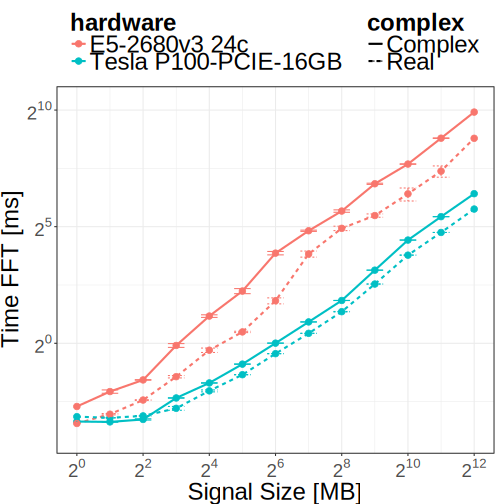
\includegraphics[width=0.45\textwidth]{figures/results_r2c_vs_c2c_a.pdf}\label{fig:r2c_vs_c2c_a}}
  \hfill
  \subfloat[real-to-complex]{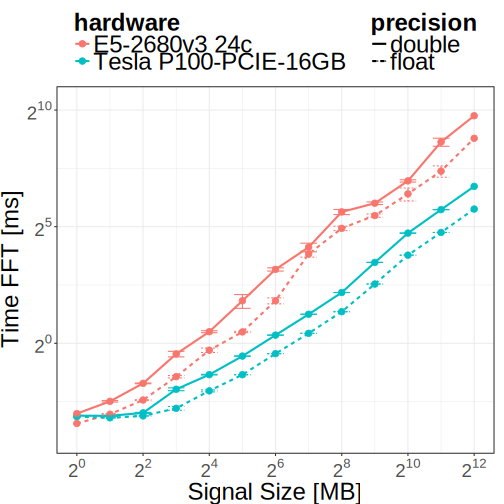
\includegraphics[width=0.45\textwidth]{figures/results_r2c_vs_c2c_b.pdf}\label{fig:r2c_vs_c2c_b}}
  \caption{Time for computing a forward FFT transform using 3D power-of-2 input signals using \fftw{} and \cufft{} on respective hardware. \cref{fig:r2c_vs_c2c_a} computes a real-to-complex transform and compares it to a complex-to-complex transform for single precision input data, whereas \cref{fig:r2c_vs_c2c_b} shows a real-to-complex transform for either single or double precision. Both figures use a log2-versus-log2 scale.}
  \label{fig:r2c_vs_c2c}
\end{figure}

\cref{fig:r2c_vs_c2c} restricts itself to larger signal sizes in order to aid the visualisation. Note that in \cref{fig:r2c_vs_c2c_a}, a data point at the same signal size does have equal shape compared to real and complex data due to complex data having double the items than real inputs. If one compares for example the entry at \SI[exponent-base=2]{e8}{\mebi\byte} for real input to the entry for \SI[exponent-base=2]{e9}{\mebi\byte} of complex type, it is clearly visible that the runtime difference amounts to \numrange{4}{8} fold regressions (note that \cref{fig:r2c_vs_c2c_a} uses a log2-log2 scale). This is equally true for \fftw{} on the CPU as well as for \cufft{} on the P100. Thus, using a complex-to-complex transform to perform an FFT on real input proves to be slower than the real-to-complex operation.

\cref{fig:r2c_vs_c2c_b} tries to answer the question, what gain can be expected if double precision is not needed for computing an FFT. On the high grade server GPU, the Nvidia Tesla P100, the performance difference remains below $2{\times}$. The results for \fftw{} vary more around \numrange{1.5}{2.5} fold regressions. 

% %% \subsection{Memory Modes}
% %% \label{ssec:mem_mode}

% The last analysis of this study is dedicated to the performance difference of inplace transforms versus out-of-place transforms. While the superficial argument is commonly mentioned that less memory is always better, it is worth having a look at the situation from data.

% \begin{figure}[!tbp]
%   \centering
%   \includegraphics[width=\textwidth]{figures/results_placiness_legend.pdf}
%   \includegraphics[width=0.45\textwidth]{figures/results_placiness_b.pdf}
%   \caption{Time for computing single-precision real-to-complex forward transforms using the 3D power-of-2 input data. The figure uses a log10-versus-log2 scale.}
%   \label{fig:placiness}
% \end{figure}

% \cref{fig:placiness} shows that in terms of performance and for large input signals, it does not matter whether the transform is performed inplace or out-of-place. There are only observable performance penalties for small input signals on the GPU.  


\section{Summary}
\label{sec:summary}
% - what can we conclude and recommend by the results?
% - what remains as part of future work?
% - issues?
% - encourage community-driven benchmark?
% - acknowledgements

With this paper, we present \gearshifft{} to the HPC community and other performance enthusiasts as an open-source, vendor-independent and free FFT benchmark suite for heterogeneous platforms. \gearshifft{} is a C++14 modular benchmark code that allows to perform forward and backward FFT transforms on various types of input data (both in shape, memory organization, precision and data type). \gearshifft{}'s design offers an extensible architecture to accomodate FFT packages with low overhead. The hallmark of \gearshifft{} is to produce reliable benchmark data that can easily be consumed by external software for visualisation and for easier reproducibility. By these design choices, we hope that \gearshifft{} appeals to both FFT practitioners, FFT library developers, HPC admins or integrators and decision makers for a wide range of use cases. To show case these capabilities, we presented a first study of common urban myths for using 3 state of the art FFT libraries, \fftw{}, \clfft{} and \cufft{}. We were able to show that the time consumed for the creation of \fftw{} plans can have non-negligible contributions to the time to solution which users of \fftw{} should be aware of. Futhermore, we compared the performance of CPU based implementations Haswell Xeon CPUs to state-of-the-art Pascal generation \nvidia{} GPUs. We were able to show that for input signal sizes of less than \SI{1}{\mebi\byte}, the CPU implementation is superior whereas for larger input data size the GPU offers better turn-around. The difference between runtimes of power-of-2, {\tt radix357} and power-of-19 shaped input data was demonstrated to be negligible for \fftw{} and non-negligible for \cufft{} transforms used in this study. We were also able to identify runtime differences when using complex versus real arrays and when comparing double versus single precision data types.     

As we warmly welcome contributions of benchmarks from various pieces of hardware, we hope to extend the \gearshifft{} repository with many more data sets of platforms used in the HPC arena of today and tomorrow. We are planning on running \gearshifft{} on non-x86 hardware to establish a basis for hardware performance comparisons. Connected to this, we plan to explore more state-of-the-art FFT libraries such as Intel IPPS, Intel MKL, AMD's rocFFT etc. We would also like to consolidate the benchmark data structure, so that many more analyses are possible than were presented in this paper both in terms of performance exploration as well as energy consumption.  

\paragraph{Acknowledgements.} The work of Matthias Werner was funded by \nvidia{} through the GPU Center of Excellence (GCOE) at the Center for Information Services and High Performance Computing (ZIH), TU Dresden, where the K20Xm and K80 GPU cluster Taurus was used. We would like to thank the Helmholtz-Zentrum Dresden-Rossendorf for providing the infrastructure to host the \nvidia{} Tesla P100 (provided by \nvidia{} for the GCOE) in the Hypnos HPC cluster. We would also like to thank the Max Planck Institute of Molecular Cell Biology and Genetics for supporting this publication by providing computing infrastructure and service staff working time.


% allows to break urls at each point
\setcounter{biburllcpenalty}{7000}
\setcounter{biburlucpenalty}{8000}
\printbibliography

\end{document}
